\section{The onset window: a persistent limitation}\label{sec:onset}

\begin{figure}[t]
\centering
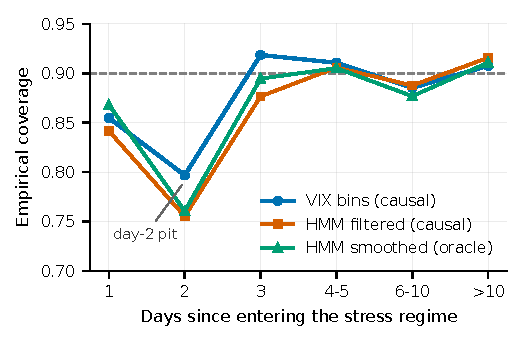
\includegraphics{figures/fig_dse_oracle.pdf}
\caption{Coverage by days since entering the stress regime, for the
causal calibrators and a noncausal calibrator given smoothed full-sample
regime memberships. The day-2 under-coverage (near
0.76--0.80 against 0.90 nominal) survives hindsight about the
regime path: onset under-coverage is score distribution shift, not regime
misdetection.}
\label{fig:dse}
\end{figure}

Every method in this paper, at every configuration, under-covers the
second day after the market enters the stress regime. The effect is worth
a section because its persistence is informative.

We conditioned on every scheme the framework can
express: finer regime partitions ($K$ up to 5), freshness subgroups
(splitting stress by days since entry), explicit transition regimes, and a
forward-looking acute group driven by the option market's own term
structure (VIX9D $>$ VIX). The acute group is genuinely useful elsewhere
(it lifts stress \emph{upper-tail} coverage to 94.8\% against the 95\%
target on the post-2012 sample), but day-2 coverage does not move. The
hindsight ablation rules out the one candidate explanation that
remains: a calibrator handed
smoothed full-sample regime memberships (one that \emph{knows},
noncausally, that the market has entered stress and will remain there)
still covers only 76\% of day-2 outcomes (Figure~\ref{fig:dse}).

The mechanics are visible in the theory. A tracker with per-observation
step size $\eta$ can move its threshold by at most $\eta \, n_t$ per day;
the day-1$\to$2 shift in the standardized score distribution during spike
onsets exceeds that budget for any $\eta$ small enough to be stable in
regime interiors (Remark~\ref{rem:notclaimed}). Larger steps trade
interior coverage for onset coverage; the adaptive aggregator, free to
make that trade under its pinball objective, declines it. Two caveats
bound this reading. The aggregator minimizes broad quantile loss, and
day-2 observations are rare; its refusal to widen may reflect that
objective's weighting rather than an information limit, which is why
Section~\ref{sec:onset-pareto} prices the trade explicitly with a
dedicated onset-widening overlay. And the one forward-looking signal we
test --- the VIX term-structure inversion, which does sharpen the
general stress tail --- carries no incremental day-2 signal; that is a
statement about this signal, not about option prices generally.

\subsection{How much evidence, and what widening would cost}
\label{sec:onset-pareto}

The onset claims rest on a small effective sample, and we state it
precisely. The market enters stress 57 times over the evaluation window,
grouped into 25 episodes more than 20 trading days apart; day-2
observations comprise 1{,}320 stock-days but only \emph{14 distinct
dates}. The day-2 coverage of the headline calibrator is $.797$, with a
date-clustered standard error of $.072$: the 95\% interval,
$[.65, .94]$, does not exclude nominal. What supports the finding
despite this is its stability, not its $t$-statistic: dropping any one
episode moves day-2 coverage only within $[.764, .848]$ (always well
below nominal in point estimate), day~1 shows the same shape
($.851 \pm .041$), and the identical pit appears in every method,
configuration, and era we examine. We present the onset window as a
robust point estimate with wide uncertainty, not a certified failure
frequency.

The mechanism is visible in the tracker's own trajectory: the issued
upper threshold averages $2.30$ standardized units on day 1 and $2.37$
on day 2 --- while the day-2 realized score mean is $1.15$, double day
1's $0.61$, with a 16.7\% upper-miss rate --- and then jumps to $3.78$
by day 3. The tracker makes the full move; it makes it one day late.

Is the window therefore uncoverable? No --- it is \emph{unpurchased}. A
deliberately crude causal overlay (multiply the issued interval by $m$
on days following a fresh stress entry, previous-day days-in-stress
1--3, no feedback into the calibrator) prices the trade: $m = 1.5$
lifts day-2 coverage from $.797$ to $.895$, at the cost of 50\% wider
onset intervals and a 2.5\% worse stress-interior interval score;
$m = 1.25$ buys $.858$ for 0.9\%. The adaptive aggregator, which
minimizes average quantile loss over all days, declines this trade
because day-2 dates are 14 out of 4{,}002. The open problem is
accordingly sharper than ``is day 2 coverable'': it is whether an
onset-aware objective can buy this coverage \emph{selectively} ---
without the crude overlay's width tax on the onsets that turn out
benign --- and whether any observable signal can time the widening
better than the entry indicator itself.

We therefore report the onset window as a persistent limitation of the
methods and signals evaluated here, rather than obscuring it inside
regime averages. Practitioners consuming these intervals should treat
the first two days of a regime transition as carrying coverage
materially below nominal, on the order of 75--85\% for a 90\% band, or
pay the overlay's explicit width price.
